\documentclass[12pt,onecolumn]{IEEEtran}

% Reading copy only -- single column, larger font, for comfortable viewing
% on an 11-inch iPad. Not the submission version; see main.tex for that.
\usepackage[margin=0.9in]{geometry}

% Match the thesis: plain Computer Modern instead of IEEEtran's default Times.
\renewcommand{\rmdefault}{cmr}
\renewcommand{\sfdefault}{cmss}
\renewcommand{\ttdefault}{cmtt}

% Bump the base text size beyond IEEEtran's 12pt ceiling for easier reading.
\makeatletter
\renewcommand{\normalsize}{\@setfontsize{\normalsize}{14}{17}}
\normalsize
\makeatother

\usepackage{amsmath}
\usepackage{booktabs}
\usepackage{graphicx}
\usepackage{url}
\renewcommand{\UrlFont}{\rmfamily}

% TODO before submission: confirm the final author list with the supervisor.
% TODO before submission: the conference website gives conflicting instructions
% about double-blind review and author names; confirm whether anonymisation is required.

\title{Per-Class QoS Prediction and SLA Violation Detection for SD-WAN}

\author{Radhika (Rishiv) Shitlani\\
School of Computer Science\\
University of Galway, Galway, Ireland}

\begin{document}

\maketitle

\begin{abstract}
Software-defined wide area networks (SD-WANs) must treat traffic classes differently, yet a single strong overall accuracy score can mask poor performance for the class that most needs scrutiny: best-effort traffic. This paper addresses two related tasks: predicting per-flow delay and detecting service-level-agreement (SLA) violations. We use 29,280 flow records from 400 BNNetSimulator runs, covering Gold, Silver, and Bronze traffic under three scheduling policies. An XGBoost regressor is evaluated with five-fold cross-validation, achieving an overall log-delay $R^2$ of 0.766, with class-specific values of 0.914, 0.908, and 0.704 for Gold, Silver, and Bronze; the corresponding SLA-violation F1 scores are 0.944, 0.720, and 0.592. Two neural alternatives, a multilayer perceptron and an FT-Transformer, reach nearly identical scores, indicating that the limiting factor is feature observability rather than model capacity. The same evaluation shows that 90th-percentile delay is only moderately predictable ($R^2$ between 0.258 and 0.657 depending on class) and that jitter is barely predictable at all ($R^2$ between 0.014 and 0.119). These results indicate that per-class evaluation is important for credible QoS prediction: a single global score would hide the large gap between how well protected and best-effort traffic can actually be predicted.
\end{abstract}

\begin{IEEEkeywords}
SD-WAN, quality of service, machine learning, XGBoost, SLA prediction, per-class evaluation
\end{IEEEkeywords}

\section{Introduction}

Software-defined wide area networking (SD-WAN) separates network control from packet forwarding, giving operators centralized control over routing and QoS policy across heterogeneous links. In practice, however, this control is typically exercised too late: operators adjust queue weights or reroute traffic only after congestion has already affected users. Predicting QoS ahead of an SLA breach could make this process proactive rather than reactive, but only if the prediction can be trusted for the traffic that most needs protecting. Gold, Silver, and Bronze traffic differ in priority, in how their delay behaves, and in what an error actually costs, so a model that appears accurate on average can still be unreliable for exactly the class most exposed to congestion.

Machine learning has already found several applications in SD-WAN research, including predicting how many virtual network functions a network will require~\cite{rahman2019autoscaling}, routing traffic based on application type~\cite{zheng2022applicationaware}, and steering traffic engineering with reinforcement learning~\cite{dinh2024safeloadbalancing,chen2025mteal}. Other work optimises SD-WAN routes and queueing policies directly from measured QoS~\cite{quang2022routing,quang2023globalqos}. These studies demonstrate that predictive or adaptive control is feasible, but none directly answer a narrower, more practical question: how accurately can continuous delay and SLA violations be predicted, separately for each traffic class, from a compact and reproducible feature set?

This paper makes three contributions:
\begin{itemize}
    \item a reproducible per-class delay-prediction study using 29,280 flows from 400 BNNetSimulator runs, reporting both regression and SLA-trigger performance separately for Gold, Silver, and Bronze traffic;
    \item a comparison across three model families, XGBoost, a multilayer perceptron, and an FT-Transformer, showing that additional model complexity does not improve per-class accuracy on this feature set; and
    \item an extension of the same evaluation to two secondary QoS targets, tail (90th-percentile) delay and jitter, establishing the limits of what a static configuration feature set can predict.
\end{itemize}

\section{Related Work}

Machine learning has been applied to several adjacent network-management tasks, though rarely to per-class QoS prediction itself. Rahman \emph{et al.} predict how many virtual network functions a system will require as load changes~\cite{rahman2019autoscaling}, while Zheng \emph{et al.} combine traffic classification with QoS-aware routing decisions~\cite{zheng2022applicationaware}; both use machine learning to inform a decision rather than to predict a continuous QoS outcome per class. For SD-WAN specifically, Quang \emph{et al.} formulate joint routing and QoS policy optimisation~\cite{quang2022routing} and later add passive available-bandwidth estimation to a two-loop controller~\cite{quang2023globalqos}; these are optimisation systems built around a fixed queueing model rather than learned predictors evaluated against ground truth. Recent work also explores safe deep reinforcement learning for load balancing~\cite{dinh2024safeloadbalancing} and multi-objective, graph-based traffic engineering~\cite{chen2025mteal}. None of these studies report how well delay or SLA compliance can be predicted separately for each priority class, which is the specific gap this paper addresses.

When labelled enterprise telemetry is unavailable, network simulators offer a reproducible alternative. BNNetSimulator generates packet-level data compatible with the modelling methodology behind RouteNet-Fermi~\cite{bnnupc2023bnnetsimulator,ferriolgalmes2022routenetfermi}, and this study uses it to examine a narrower, more practical question than the wider literature addresses: can static configuration and path features alone support reliable, class-specific QoS prediction? XGBoost is used as the primary model because gradient-boosted trees remain strong performers on small-to-medium tabular datasets~\cite{grinsztajn2022trees,shwartzziv2022tabular}, train comparatively quickly, provide inexpensive split-based feature-importance measures, and support efficient Tree SHAP explanations.

\section{Methodology}

\subsection{Dataset and QoS Classes}

The dataset was generated with the official BNNetSimulator container~\cite{bnnupc2023bnnetsimulator} and contains 29,280 source-destination flow records from 400 simulation runs, with 30--132 flows per run. Traffic is divided into three classes: Gold (4,592 rows, highest priority), Silver (8,991 rows, interactive traffic), and Bronze (15,697 rows, best effort). The experiments span strict priority, WFQ, and deficit round robin scheduling across four scenarios: fixed WFQ weights, randomised WFQ profiles, and two mixed-policy scenarios with skewed and equal class proportions. The generator was configured to avoid deliberate near-saturation, so the results below should be read as a controlled study of per-class prediction rather than a stress test of a saturated production network.

Each input row includes the traffic class, offered bandwidth, traffic distribution, route length, network size, maximum average load, link bandwidth, scheduling policy, class queue weight, and minimum class weight. The prediction target is the natural logarithm of average delay in seconds. Any field that would leak the answer, namely raw delay, jitter, packet loss, delay percentiles, achieved bandwidth, the scenario label, and the simulation identifier itself, is excluded from the feature matrix. Missing numeric values are median-imputed and categorical variables are one-hot encoded, both computed separately within each training fold to avoid leakage.

\subsection{Prediction and Evaluation}

The primary regressor is XGBoost, configured with 200 trees, a maximum depth of four, a learning rate of 0.05, and row and feature subsampling both set to 0.9. Because the model is trained on log delay, predictions are converted back to milliseconds before being reported, so that the error values carry operational meaning. Performance is measured using mean absolute error (MAE) on the millisecond scale and $R^2$ on log delay.

Five-fold cross-validation is used, with folds constructed by randomly shuffling the full set of flow rows under a fixed random seed. Preprocessing and model fitting are refit independently within every fold, and every reported metric is derived from out-of-fold predictions rather than training predictions.

Continuous delay predictions are also converted into binary SLA-violation triggers, using thresholds of 30, 50, and 60 ms for Gold, Silver, and Bronze respectively. Precision indicates how much a trigger can be trusted once it fires, recall indicates how many real violations are actually caught, and F1 balances the two. The Bronze threshold was derived from an exploratory sensitivity sweep rather than a fixed requirement, and should be read as a reasonable operating point rather than a universal SLA value.

The same evaluation protocol and leakage-safe feature exclusions are reused for two secondary targets, 90th-percentile delay and jitter, evaluated directly in milliseconds since that is the scale most relevant to the operational question.

\subsection{Reproducibility}

Data generation, preprocessing, evaluation, and plotting are implemented as separate, reusable Python scripts. Randomised estimators use a fixed seed (42), and every reported metric is derived from out-of-fold predictions rather than training predictions, ensuring that no result is inflated by the model having already seen the row it is scored on. The generated dataset, experiment scripts, and result tables are available in the project repository; a permanent archival identifier will be added for the camera-ready version.

\section{Results}

\subsection{Per-Class Delay and SLA Prediction}

Table~\ref{tab:main} reports the primary results. Overall $R^2$ is 0.766, with a delay-scale MAE of 13.52 ms, though this single figure conceals a substantial class-dependent gap. Gold and Silver are predicted accurately ($R^2=0.914$ and 0.908), while Bronze falls to 0.704 and its MAE nearly triples to 20.68 ms. This pattern is consistent with protected traffic being shaped primarily by stable topology and scheduler configuration, which the static features capture well, while best-effort delay may also depend on transient contention that these features cannot observe.

\begin{table}[t]
\caption{Five-Fold Cross-Validation Results}
\label{tab:main}
\centering
\setlength{\tabcolsep}{3.5pt}
\begin{tabular}{lrrrrr}
\toprule
Class & MAE & $R^2$ & Prec. & Recall & F1 \\
 & (ms) & & & & \\
\midrule
Gold   & 3.05  & 0.914 & 0.994 & 0.899 & 0.944 \\
Silver & 3.48  & 0.908 & 0.823 & 0.639 & 0.720 \\
Bronze & 20.68 & 0.704 & 0.619 & 0.568 & 0.592 \\
\bottomrule
\end{tabular}
\end{table}

Gold's SLA trigger maintains a very high precision of 0.994: the model is correct 99.4\% of the time when it predicts a Gold violation. This is an important property for any controller that acts on such predictions, since false positives on the highest-priority class could trigger unnecessary intervention. Silver and Bronze are noticeably less reliable, particularly on recall, and Bronze's F1 of 0.592 illustrates an important point: a regressor that appears accurate in aggregate does not automatically translate into a strong SLA-violation detector for best-effort traffic.

\subsection{Model Complexity and Feature Evidence}

A comparison across model families, shown in Table~\ref{tab:models}, found nearly identical overall scores for XGBoost ($R^2=0.766$), a multilayer perceptron (0.766), and an FT-Transformer (0.762). All three model families reach essentially the same Bronze ceiling, and the FT-Transformer trails only marginally on Gold and Silver, with no gap exceeding 0.014 $R^2$. This is a clear signal that additional neural complexity provides little benefit here, since it cannot compensate for short-timescale traffic information absent from the feature set. XGBoost is retained as the model of choice for the remainder of the study because it matches the neural models while remaining interpretable and far less costly to train.

\begin{table}[t]
\caption{Row-Wise Model Comparison}
\label{tab:models}
\centering
\setlength{\tabcolsep}{4pt}
\begin{tabular}{lrrrr}
\toprule
Model & Overall & Gold & Silver & Bronze \\
 & $R^2$ & $R^2$ & $R^2$ & $R^2$ \\
\midrule
XGBoost        & 0.766 & 0.914 & 0.908 & 0.704 \\
MLP            & 0.766 & 0.912 & 0.908 & 0.705 \\
FT-Transformer & 0.762 & 0.900 & 0.898 & 0.703 \\
\bottomrule
\end{tabular}
\end{table}

SHAP values for the final XGBoost model support this conclusion (Fig.~\ref{fig:shap}). Route length dominates: additional hops push predictions toward higher log delay, while shorter paths pull them down. Network size and traffic class follow at some distance, with queue weights and scheduling-policy indicators contributing comparatively little on their own. These represent associations learned within the simulator rather than causal estimates, but they tell a consistent story: the model relies primarily on stable path structure. This structure is genuinely informative for protected Gold and Silver flows, but the weaker Bronze results suggest that it does not fully capture transient contention affecting best-effort delay.

\begin{figure}[t]
\centering
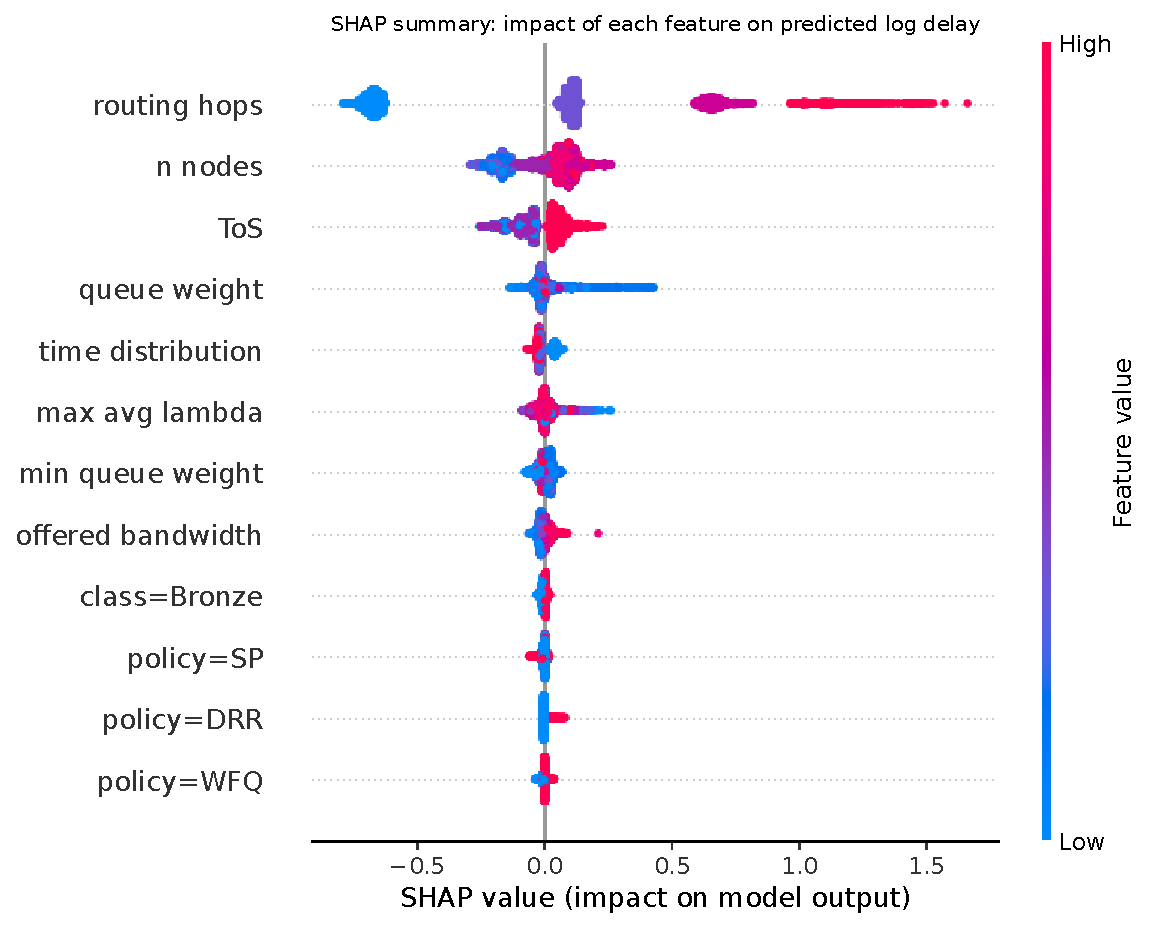
\includegraphics[width=0.85\textwidth]{figures/shap_summary.pdf}
\caption{SHAP summary for the XGBoost log-delay model; colour denotes feature value.}
\label{fig:shap}
\end{figure}

\subsection{Tail Delay and Jitter}

Table~\ref{tab:secondary} applies the same evaluation to two secondary QoS targets. Tail delay is noticeably harder to predict than average delay: Gold and Silver reach only moderate $R^2$ values of 0.635 and 0.657, and Bronze falls much further to 0.258, with its MAE climbing to 38.22 ms. This is expected, since the 90th percentile captures rarer, more variable congestion events than the mean, and the same gap that separates Bronze from Gold and Silver on average delay is amplified in the tail.

Jitter is very weakly predicted across every class, with $R^2$ ranging only from 0.014 (Bronze) to 0.119 (Gold). This is a meaningful finding rather than a modelling failure: the feature set describes static network configuration, such as queue weights, scheduling policy, and offered bandwidth, and these features determine mean delay well but do not capture the moment-to-moment traffic burstiness that drives jitter. Predicting jitter reliably would require dynamic features such as instantaneous queue occupancy or inter-arrival time statistics, neither of which is present in this dataset. Together, these results sharpen the boundary of what this feature set can convey: it describes average delay well, tail delay only partially, and moment-to-moment delay variation barely at all.

\begin{table}[t]
\caption{Per-Class Results for Secondary QoS Targets}
\label{tab:secondary}
\centering
\setlength{\tabcolsep}{5pt}
\begin{tabular}{llrr}
\toprule
Target & Class & MAE (ms) & $R^2$ \\
\midrule
Delay p90 & Gold    & 6.64  & 0.635 \\
          & Silver  & 7.29  & 0.657 \\
          & Bronze  & 38.22 & 0.258 \\
\midrule
Jitter    & Gold    & 0.14 & 0.119 \\
          & Silver  & 0.16 & 0.084 \\
          & Bronze  & 3.11 & 0.014 \\
\bottomrule
\end{tabular}
\end{table}

\section{Discussion and Limitations}

The central finding here is not simply that delay is predictable, but that its predictability depends heavily on the traffic class and on which target is being predicted. Route length, network size, and traffic class encode stable structure, and this structure explains protected average delay well. Bronze, having the lowest service priority, may be more exposed to bursts and queue occupancy that the current features do not measure. The weak jitter results reinforce this interpretation: increasing model complexity cannot recover transient state that is absent from the features.

Several limitations should temper these claims. First, no real-world enterprise SD-WAN dataset with labelled QoS metrics was available for this work, so the results rely on data generated by BNNetSimulator rather than measured on a live network. The evaluation measures performance on held-out flow records generated by BNNetSimulator; it does not establish transfer to a real enterprise SD-WAN. Second, the feature set is entirely static: telemetry such as instantaneous queue occupancy, recent arrival-rate windows, and recent loss would be required to model transient behaviour, and none of this is present here. Third, the SLA thresholds used are experimental operating points rather than contractual values drawn from a real deployment. Future work should add dynamic traffic features, such as instantaneous queue depth or inter-arrival time statistics, to improve Bronze delay, tail delay, and jitter prediction, and should validate the approach against real controller telemetry.

\section{Conclusion}

This paper presented a per-class evaluation of QoS prediction for SD-WAN-like networks. XGBoost predicts Gold and Silver average delay accurately, is noticeably less reliable for Bronze, and is only weakly predictive for jitter. Comparing XGBoost against a multilayer perceptron and an FT-Transformer shows that additional model complexity does not improve on any of these results, indicating that the limiting factor is feature observability rather than model capacity. The broader implication is straightforward: trustworthy AI-assisted QoS prediction requires class-aware metrics and an honest account of what static network features can and cannot support.

\bibliographystyle{IEEEtran}
\bibliography{references}

\end{document}
